\chapter{بخش چهارم}
در این بخش به طراحی کنترل‌کننده از خانواده  PID به کمک برنامه optimPID متلب پرداخته شده است که در آن کنترل‌کننده PIDF به روش های مختلف بهینه سازی امتحان و طراحی شده است که برای طراحی نیز دو حالت با بلوک اشباع و بدون بلوک اشباع در نظر گرفته شده و برای هر دو حالت کنترل‌کنندهطراحی شده است که شکل مدار باز سیستم مورد استفاده در این برنامه برای هر یک از حالت های با / بدون اشباع به صورت زیر است:

\begin{figure}[H]
	\centering
	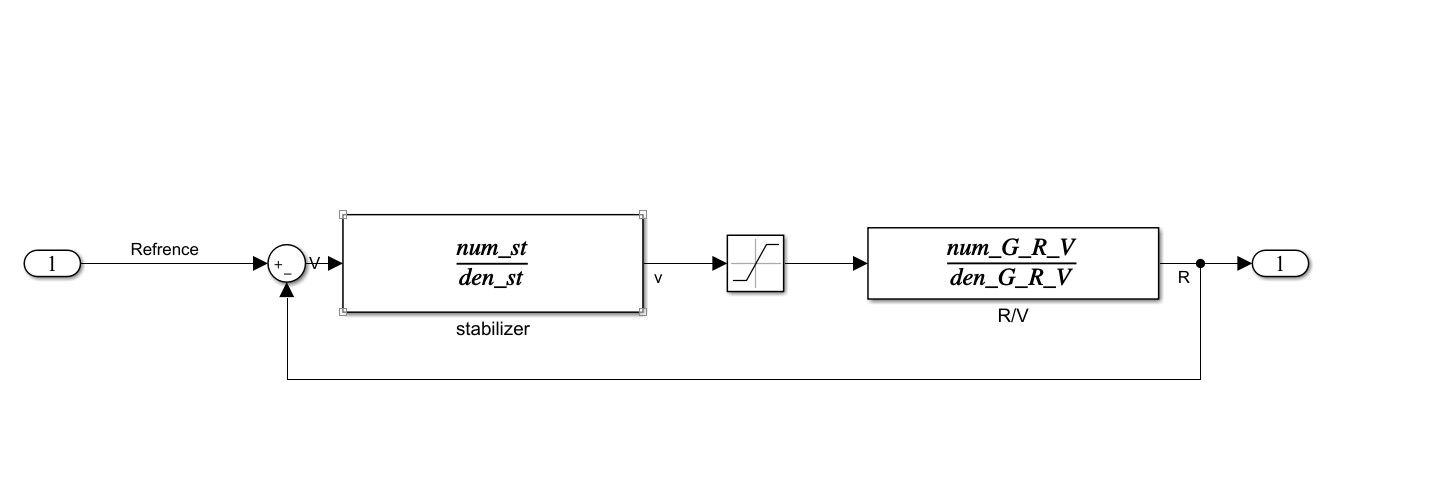
\includegraphics[width=12cm]{../Figure/P_IV/OL_optimpid_with_sat.jpg}
	\caption{بلوک دیاگرام مدار باز سیستم استفاده شده در optimpid در حالت با اشباع}
\end{figure}

\begin{figure}[H]
	\centering
	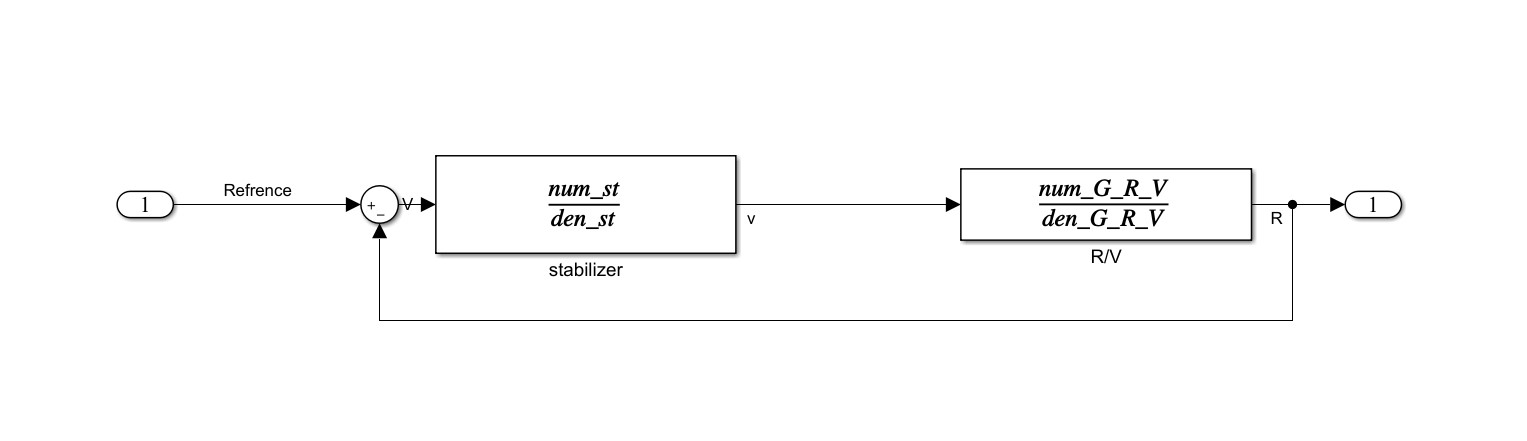
\includegraphics[width=12cm]{../Figure/P_IV/OL_optimpid_without_sat.jpg}
	\caption{بلوک دیاگرام مدار باز سیستم استفاده شده در optimpid در حالت بدون اشباع}
\end{figure}



نمودار مربوط به ورودی مرجع 0.5 متر برای هر کدام از کنترل‌کنندههای طراحی شده به صورت زیر است:
\begin{figure}[H]
	\centering
	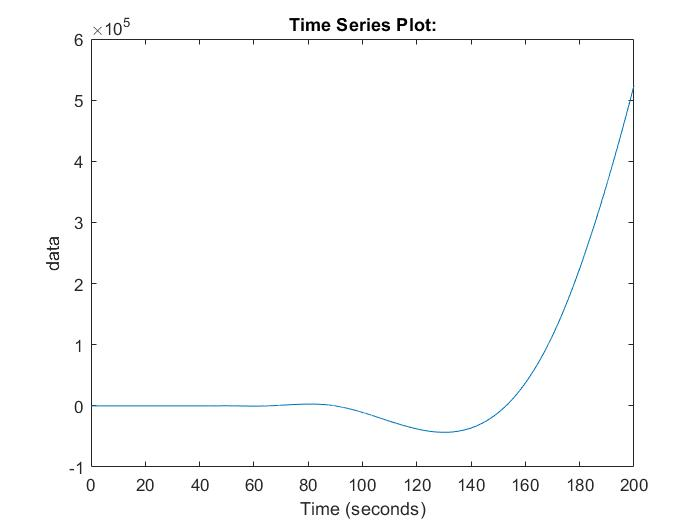
\includegraphics[width=12cm]{../Figure/P_IV/PID_IAE_with_sat.jpg}
	\caption{کنترل‌کننده PIDF طراحی شده در برنامه optimpid متلب برای حالت همراه با بلوک اشباع و با روش بهینه سازی IAE}
\end{figure}

\begin{figure}[H]
	\centering
	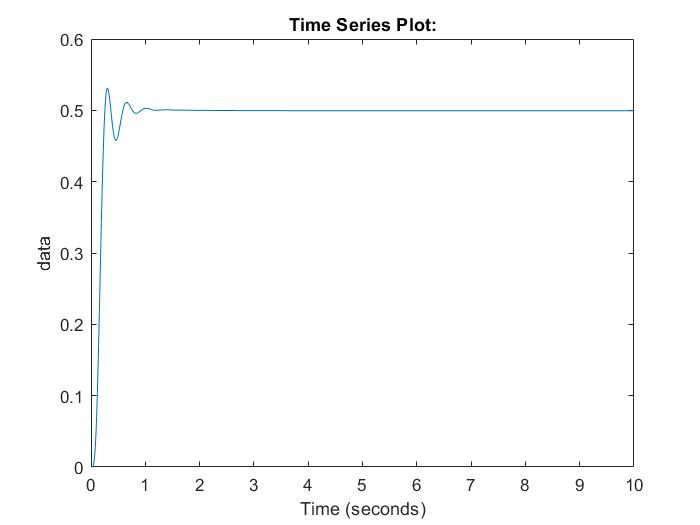
\includegraphics[width=12cm]{../Figure/P_IV/PID_IAE_without_sat.jpg}
	\caption{کنترل‌کننده PIDF طراحی شده در برنامه optimpid متلب برای حالت همراه بدون بلوک اشباع و با روش بهینه سازی IAE}
\end{figure}

\begin{figure}[H]
	\centering
	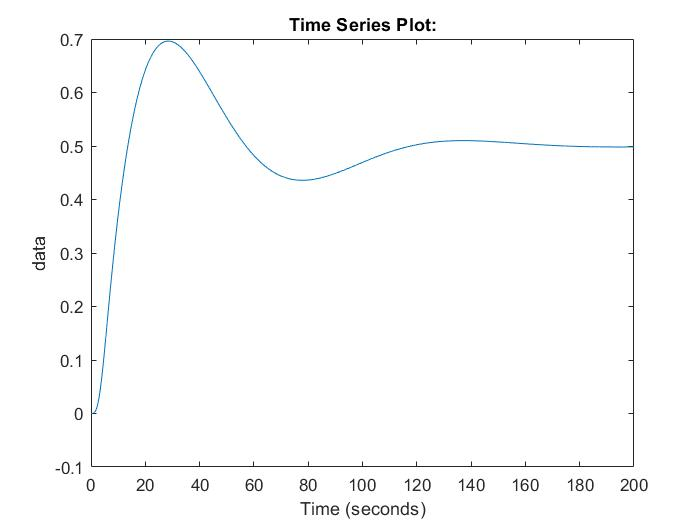
\includegraphics[width=12cm]{../Figure/P_IV/PID_ISE_with_sat.jpg}
	\caption{کنترل‌کننده PIDF طراحی شده در برنامه optimpid متلب برای حالت همراه با بلوک اشباع و با روش بهینه سازی ISE}
\end{figure}

\begin{figure}[H]
	\centering
	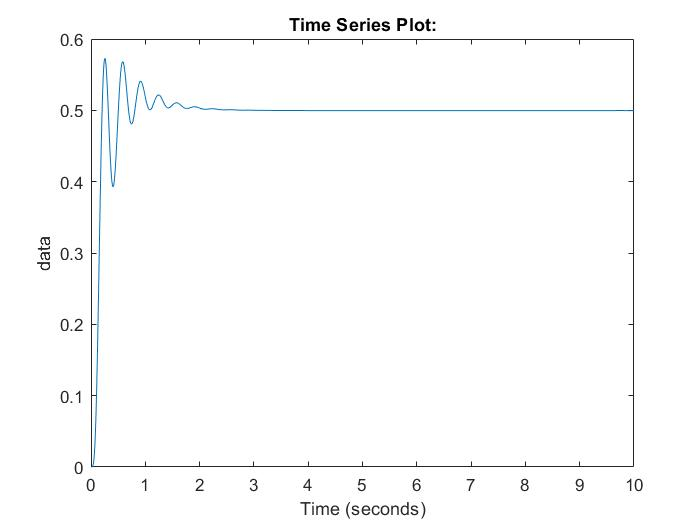
\includegraphics[width=12cm]{../Figure/P_IV/PID_ISE_without_sat.jpg}
	\caption{کنترل‌کننده PIDF طراحی شده در برنامه optimpid متلب برای حالت همراه بدون بلوک اشباع و با روش بهینه سازی ISE}
\end{figure}

\begin{figure}[H]
	\centering
	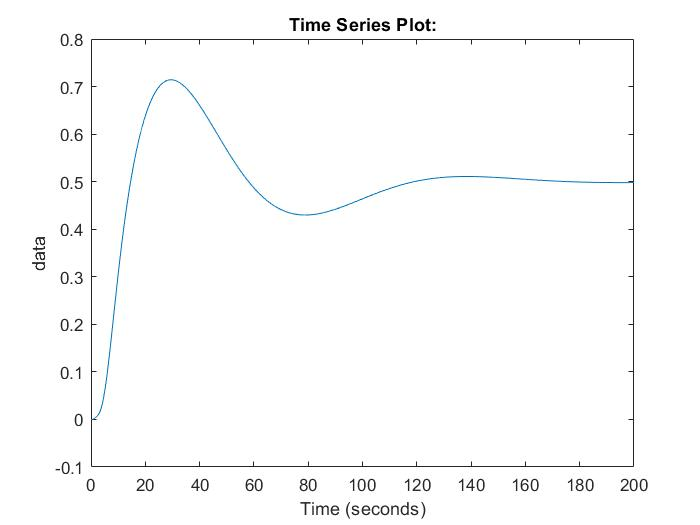
\includegraphics[width=12cm]{../Figure/P_IV/PID_IT2AE_with_sat.jpg}
	\caption{کنترل‌کننده PIDF طراحی شده در برنامه optimpid متلب برای حالت همراه با بلوک اشباع و با روش بهینه سازی \lr{IT2AE}}
\end{figure}

%

\begin{figure}[H]
	\centering
	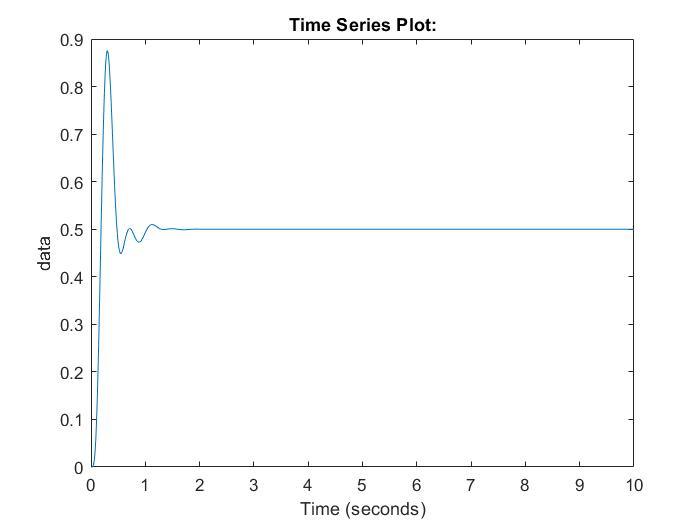
\includegraphics[width=12cm]{../Figure/P_IV/PID_IT2AE_without_sat.jpg}
	\caption{کنترل‌کننده PIDF طراحی شده در برنامه optimpid متلب برای حالت همراه بدون بلوک اشباع و با روش بهینه سازی \lr{IT2AE}}
\end{figure}

\begin{figure}[H]
	\centering
	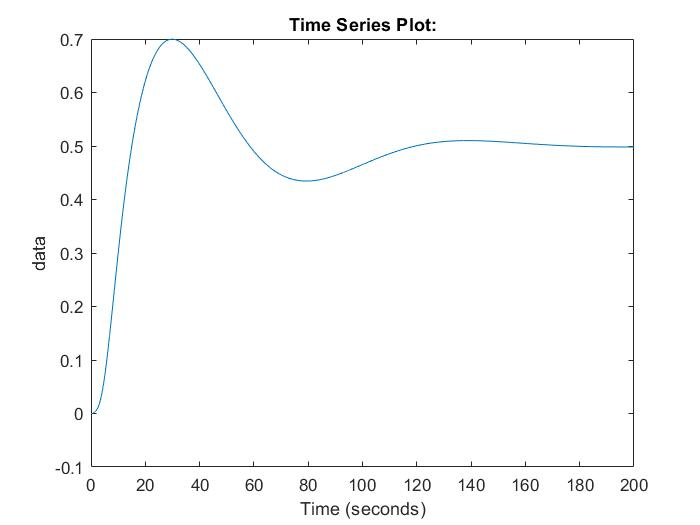
\includegraphics[width=12cm]{../Figure/P_IV/PID_IT2SE_with_sat.jpg}
	\caption{کنترل‌کننده PIDF طراحی شده در برنامه optimpid متلب برای حالت همراه با بلوک اشباع و با روش بهینه سازی \lr{IT2SE}}
\end{figure}

\begin{figure}[H]
	\centering
	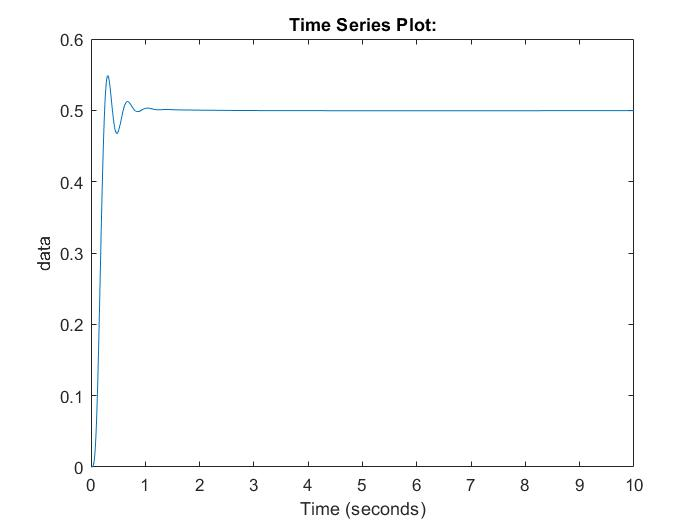
\includegraphics[width=12cm]{../Figure/P_IV/PID_IT2SE_without_sat.jpg}
	\caption{کنترل‌کننده PIDF طراحی شده در برنامه optimpid متلب برای حالت همراه بدون بلوک اشباع و با روش بهینه سازی \lr{IT2SE}}
\end{figure}



\begin{figure}[H]
	\centering
	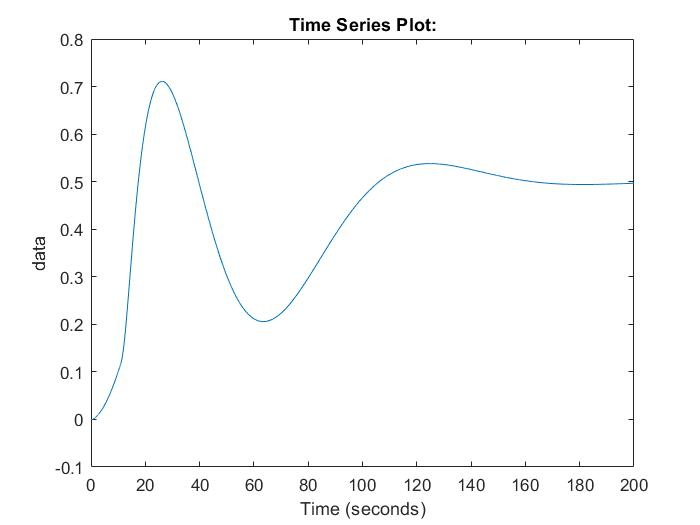
\includegraphics[width=12cm]{../Figure/P_IV/PID_ITAE_with_sat.jpg}
	\caption{کنترل‌کننده PIDF طراحی شده در برنامه optimpid متلب برای حالت همراه با بلوک اشباع و با روش بهینه سازی ITAE}
\end{figure}
%

\begin{figure}[H]
	\centering
	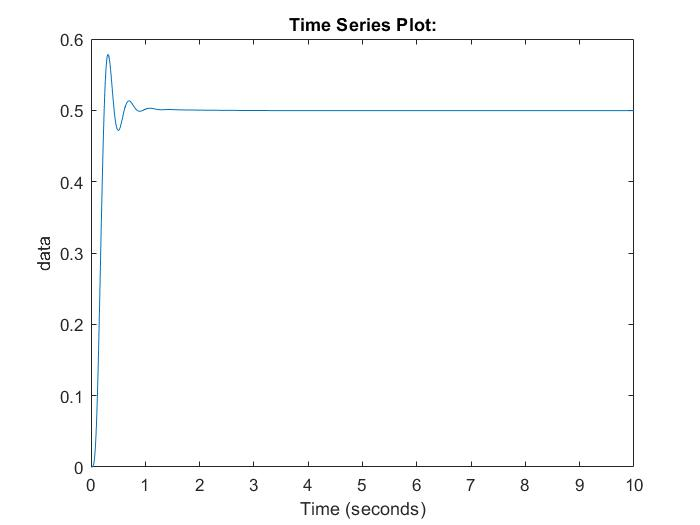
\includegraphics[width=12cm]{../Figure/P_IV/PID_ITAE_without_sat.jpg}
	\caption{کنترل‌کننده PIDF طراحی شده در برنامه optimpid متلب برای حالت همراه بدون بلوک اشباع و با روش بهینه سازی ITAE}
\end{figure}


\begin{figure}[H]
	\centering
	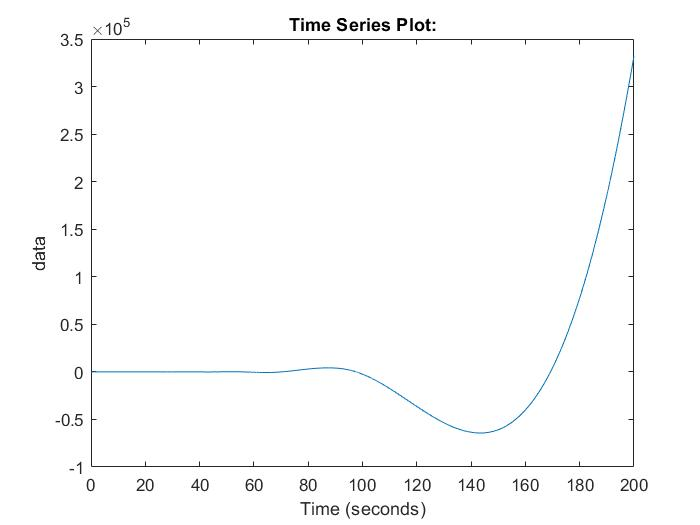
\includegraphics[width=12cm]{../Figure/P_IV/PID_ITSE_with_sat.jpg}
	\caption{کنترل‌کننده PIDF طراحی شده در برنامه optimpid متلب برای حالت همراه با بلوک اشباع و با روش بهینه سازی ITAE}
\end{figure}

%

\begin{figure}[H]
	\centering
	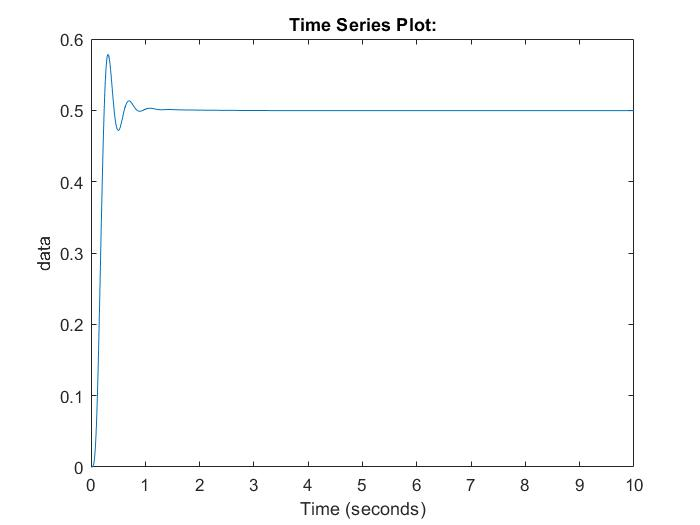
\includegraphics[width=12cm]{../Figure/P_IV/PID_ITAE_without_sat.jpg}
	\caption{‌کنترل‌کننده PIDF طراحی شده در برنامه optimpid متلب برای حالت همراه بدون بلوک اشباع و با روش بهینه سازی ITSE}
\end{figure}



%
همانطور که ملاحظه می شود با اضافه شدن بلوک اشباع به سیستم مدار باز برنامه قادر به طراحی کنترل‌کنندهی که زمان نشست ان کمتر از 6 ثانیه باشد نمی باشد و بهترین کنترل‌کننده های طراحی شده توسط برنامه برای سیستم با بلوک اشباع دارای زمان نشست بیشتر از 100 ثانیه می باشند.
%
%
%
%
%
